
\chapter{Extensions and Changes}
\label{ch:otherChanges}


%\cite{Swat:2016qf, MLXTRANforMonolix:2014}

%%%%%%%%%%%%%%%%%%%%%%%%%%%%%%%%%%%%%%%%%%%%%%%%%%%%%%%%%%%%%%%%%%%%%%
\section{General}

\subsection{Box-Cox 2}
\label{sec:BoxCox2Trafo}

The Box-Cox Transformation, \cite{BoxCox:1964}, is used to transform data to 
an approximate normal distribution and the most common version, for $y \geq 0$ 
was introduced in version 0.7, \cite{Swat:2015b}. Now we introduce 
also a two-parameter version capable to deal with negative values, which was 
proposed in the original paper by Box \& Cox
\begin{align}
y^{(\mathbf{\lambda})} = \left\{ \begin{array}{rcl}  \dfrac{(y+\lambda_2)^{\lambda_1} -1}{\lambda_1} & \mbox{for} & \lambda_1 \neq 0 \\ 
\log(y + \lambda_2) & \mbox{for} & \lambda_1 = 0 \end{array}\right. \label{eq:BC2}
\end{align}

In PharmML, appliedd to a simple observation model, it reads
\lstset{language=XML}
\begin{lstlisting}
        <Standard symbId="Y">
            <Transformation type="BoxCox2">
                <Parameter>
                    <ct:Assign>
                        <ct:SymbRef symbIdRef="lambda1"/>
                    </ct:Assign>
                </Parameter>
                <Parameter>
                    <ct:Assign>
                        <ct:SymbRef symbIdRef="lambda2"/>
                    </ct:Assign>
                </Parameter>
            </Transformation>
            <Output>
                <ct:SymbRef blkIdRef="sm1" symbIdRef="f"/>
            </Output>
            <ErrorModel>
                <ct:Assign>
                    <ct:SymbRef symbIdRef="a"/>
                </ct:Assign>
            </ErrorModel>
            <ResidualError>
                <ct:SymbRef symbIdRef="eps"/>
            </ResidualError>
        </Standard>
\end{lstlisting}

\paragraph{Note} \marginpar{\HandCuffLeft} that the assumption is that the sequence matters 
in the code above and that the first and second parameter correspond 
to $\lambda_1$ and $\lambda_2$ in  eq.(\ref{eq:BC2}), respectively.

%%%%%%%%%%%%%%%%%%%%%%%%%%%%
\subsection{User-defined transformations}
\label{sec:userDefTrafo}
There are many transformations one could apply, see e.g. \cite{Sakia:1992fu},
and to cover all is simply impossible. Therefore, we introduce simple extension 
mechanism allowing to implement virtually any conceivable transformation 
and realising already existing features. 

\bigskip
The \xelem{Transformation type="..."} element gets 
\begin{itemize}
\item 
new value \textit{userDefined} for the \xatt{type} attribute 
\end{itemize}
which can be used for such cases. In the following
we show how the extended Box-Cox transformation, \textit{Box-Cox 2}, 
introduced in the previous section, could be implemented using this option.

\begin{itemize}
\item 
it starts with the implementation of the Box-Cox 2 function expressed by 
the eq.(\ref{eq:BC2}), called \textit{BoxCox2Func}, using the \xelem{FunctionDefinition} 
structure. The following code snippet shows how this is done.

\lstset{language=XML}
\begin{lstlisting}
    <ct:FunctionDefinition symbId="BoxCox2Func">
        <ct:FunctionArgument symbId="lambda1"/>
        <ct:FunctionArgument symbId="lambda2"/>
        <ct:FunctionArgument symbId="y"/>
        <ct:Definition>
            <ct:Assign>
                <math:Piecewise>
                    <!-- omitted Box-Cox 2 formula for brevity -->
                </math:Piecewise>
            </ct:Assign>
        </ct:Definition>
    </ct:FunctionDefinition>
\end{lstlisting}

%                    <math:Piece>
%                        <math:Binop op="divide">
%                            <math:Binop op="minus">
%                                <math:Binop op="power">
%                                    <math:Binop op="plus">
%                                        <ct:SymbRef symbIdRef="y"/>
%                                        <ct:SymbRef symbIdRef="lambda2"/>
%                                    </math:Binop>
%                                    <ct:SymbRef symbIdRef="lambda1"/>
%                                </math:Binop>
%                                <ct:Real>1</ct:Real>
%                            </math:Binop>
%                            <ct:SymbRef symbIdRef="lambda1"/>
%                        </math:Binop>
%                        <math:Condition>
%                            <math:LogicBinop op="neq">
%                                <ct:SymbRef symbIdRef="lambda1"/>
%                                <ct:Real>0</ct:Real>
%                            </math:LogicBinop>
%                        </math:Condition>
%                    </math:Piece>
%                    <math:Piece>
%                        <math:Uniop op="log">
%                            <math:Binop op="plus">
%                                <ct:SymbRef symbIdRef="y"/>
%                                <ct:SymbRef symbIdRef="lambda2"/>
%                            </math:Binop>
%                        </math:Uniop>
%                        <math:Condition>
%                            <math:LogicBinop op="eq">
%                                <ct:SymbRef symbIdRef="lambda1"/>
%                                <ct:Real>0</ct:Real>
%                            </math:LogicBinop>
%                        </math:Condition>
%                    </math:Piece>

\item
this function can then be used to define the following additive observation model
applied to the transformed data.
\begin{align}
h(Cc_{obs}) = h(Cc) + a \times \epsilon \nonumber
\end{align}
with $h \equiv \text{'Box-Cox 2' transformation}$

\lstset{language=XML}
\begin{lstlisting}
      <ObservationModel blkId="userDefinedTrafoModel">
            <ContinuousData>
                <PopulationParameter symbId="LAMBDA1"/>
                <PopulationParameter symbId="LAMBDA2"/>

                <RandomVariable symbId="eps">
                    <Distribution>
                        <po:ProbOnto name="StandardNormal1"/>
                    </Distribution>
                </RandomVariable>
                
                <Standard>
                    <Transformation type="userDefined">
                        <math:FunctionCall>
                            <ct:SymbRef symbIdRef="BoxCox2Func"/>
                            <math:FunctionArgument symbId="lambda1">
                                <ct:SymbRef symbIdRef="LAMBDA1"/>
                            </math:FunctionArgument>
                            <math:FunctionArgument symbId="lambda2">
                                <ct:SymbRef symbIdRef="LAMBDA2"/>
                            </math:FunctionArgument>
                            <math:FunctionArgument symbId="y">
                                <ct:SymbRef blkIdRef="sm1" symbIdRef="Cc"/>
                            </math:FunctionArgument>
                        </math:FunctionCall>
                    </Transformation>
                    <Output>
                        <ct:SymbRef blkIdRef="sm1" symbIdRef="Cc"/>
                    </Output>
                    <ErrorModel>
                        <ct:Assign>
                            <ct:SymbRef symbIdRef="a"/>
                        </ct:Assign>
                    </ErrorModel>
                    <ResidualError>
                        <ct:SymbRef symbIdRef="eps"/>
                    </ResidualError>
                </Standard>
                
            </ContinuousData>
        </ObservationModel>
\end{lstlisting}

\end{itemize}


%%%%%%%%%%%%%%%%%%%%%%%%%%%%
\subsection{User-defined distributions}
\label{sec:userDefDistros}

Similarly to user-defined functions, there are situations where we might 
be interested in declarations of distributions not covered by the ProbOnto
database, \cite{Swat:2016qf}. 
We start here with two motivating examples and explain later the new supporting
elements in PharmML.

\paragraph{Example 1} We consider here a density function describing insulin release,
\cite{Grodsky:1972kq}, which reads
\begin{align}
f(x) = X_{max} \frac{k \,C \,x^{k-1}}{(C + x^k)^2} \nonumber
\end{align}

As before, section \ref{sec:userDefTrafo}, we define first the density function
in question using the \xelem{FunctionDefinition} element
\lstset{language=XML}
\begin{lstlisting}
    <!-- User-defined density function - Grodsky 1972 -->
    <ct:FunctionDefinition symbId="GrodskyPDF">
        <ct:FunctionArgument symbId="Xmax"/>
        <ct:FunctionArgument symbId="k"/>
        <ct:FunctionArgument symbId="C"/>
        <ct:FunctionArgument symbId="x"/>
        <ct:Definition>
            <ct:Assign>
                <!-- we omit the implementation of the following RHS expression  -->
                <!-- Xmax * k * C x^{k-1} / (C + x^k)^2  -->
            </ct:Assign>
        </ct:Definition>
    </ct:FunctionDefinition>
\end{lstlisting}
which can then be used to declare a distribution model of a variable, parameter 
or covariate. Here we use it in an observation model.

\lstset{language=XML}
\begin{lstlisting}
        <ObservationModel blkId="Grodsky1972">
            <ContinuousData>
                <General symbId="Y">
                    <Distribution>
                        <UserDefDistribution type="PDF">
                            <ct:Assign>
                                <math:FunctionCall>
                                    <ct:SymbRef symbIdRef="GrodskyPDF"/>
                                    <math:FunctionArgument symbId="Xmax">
                                        <ct:SymbRef symbIdRef="Xmax"/>
                                    </math:FunctionArgument>
                                    <!-- omitted argument mapping for k, C, theta and x -->
                                </math:FunctionCall>
                            </ct:Assign>
                        </UserDefDistribution>
                    </Distribution>
                </General>
            </ContinuousData>
        </ObservationModel>
\end{lstlisting}

\paragraph{Example 2} Yet another example is a user-defined covariate distribution definition, which reads
\lstset{language=XML}
\begin{lstlisting}
            <Covariate symbId="testCovariate">
                <Categorical>
                    <Category catId="cat1"/>
                    <Category catId="cat2"/>
                    <Distribution>
                        <UserDefDistribution type="PMF">
                            <ct:Assign>
                                <!-- dummy function -->
                                <ct:Real>1</ct:Real>
                            </ct:Assign>
                        </UserDefDistribution>
                    </Distribution>
                </Categorical>
            </Covariate>
\end{lstlisting}


\subsubsection*{PharmML support}
When declaring a ProbOnto distribution, e.g. the standard normal,
it is sufficient to declare its  code name, i.e.
\lstset{language=XML}
\begin{lstlisting}
                    <Distribution>
                        <po:ProbOnto name="StandardNormal1"/>
                    </Distribution>
\end{lstlisting}

Instead, as shown in the examples above, we use the introduced
\xelem{UserDefDistribution type="..."} element with attribute informing 
the target tool about the type of the defining function which can be one of the
following values \{\emph{CDF}, \emph{PDF}, \emph{PMF}, \emph{HF}, \emph{SF}\}
as the snippet below illustrates
\lstset{language=XML}
\begin{lstlisting}
                    <Distribution>
                        <UserDefDistribution type="PDF">
                            <ct:Assign>
                                    <!-- omitted details -->
                            </ct:Assign>
                        </UserDefDistribution>
                    </Distribution>
\end{lstlisting}
Within the \xelem{Assign} tag, we can either declare the function of interest 
directly, Example 1, or using \xelem{FunctionCall},  Example 2, to refer to a previously 
defined function. Attribute \xatt{type} is mandatory.



%%%%%%%%%%%%%%%%%%%%%%%%%%%%
\subsection{Accessing ODE initial condition values}
\label{subsec:initialValue}
It is sometimes desirable to refer or to use the initial condition values 
of an ODE defined variable as suggested in the NT2MDL converter 
report \cite{nt2mdl:2016}. The following NMTRAN code illustrates 
one such example
\lstset{language=NM}
\begin{lstlisting}
	A_0(6)=Ccol ; Colistin	
	IF(A_0(6).EQ.0.04162.AND.TIME.LT.8) KE2 = 0.059
\end{lstlisting}
and the PharmML implementation reads as follows. 
The ODE for A6 is shown abbreviated for clarity and only the 
initial value assignment is fully displayed 
\lstset{language=XML}
\begin{lstlisting}
    <StructuralModel blkId="sm1">
	...
        <ct:DerivativeVariable symbId="A6">
            <ct:Assign>
                <!-- RHS of the ODE omitted -->
            </ct:Assign>
            <ct:InitialCondition>
                <ct:InitialValue>
                    <ct:Assign>
                        <ct:SymbRef symbIdRef="Ccol"/>
                    </ct:Assign>
                </ct:InitialValue>
            </ct:InitialCondition>
        </ct:DerivativeVariable>
        ...
    </StructuralModel>
\end{lstlisting}
Then the conditional \emph{KE2} parameter assignment reads
\lstset{language=XML}
\begin{lstlisting}
    <ParameterModel blkId="pm1">
    	....
        <IndividualParameter symbId="KE2">
            <ct:Assign>
                <math:Piecewise>
                    <math:Piece>
                        <ct:Real>0.059</ct:Real>
                        <math:Condition>
                            <math:LogicBinop op="and">
                                <math:LogicBinop op="eq">
                                    <ct:InitialValue>
                                        <ct:Assign>
                                            <ct:SymbRef blkIdRef="sm1" symbIdRef="A6"/>
                                        </ct:Assign>
                                    </ct:InitialValue>
                                    <ct:Real>0.04162</ct:Real>
                                </math:LogicBinop>
                                <math:LogicBinop op="lt">
                                    <ct:SymbRef symbIdRef="t"/>
                                    <ct:Real>8</ct:Real>
                                </math:LogicBinop>
                            </math:LogicBinop>
                        </math:Condition>
                    </math:Piece>
                </math:Piecewise>
            </ct:Assign>
        </IndividualParameter>
        ...
    <ParameterModel blkId="pm1">
\end{lstlisting}


%%%%%%%%%%%%%%%%%%%%%%%%%%%%
\subsection{Selecting vector/matrix elements}
\label{sec:EndIndex}

New element 
\begin{itemize}
\item 
\xelem{EndIndex} 
\end{itemize}
has been added to \xelem{VectorSelector}
to facilitate efficient selecting operations applied to vectors and matrices.
Two examples illustrate its use

\subsubsection*{Example 1: Picking last element of the 1st column}
In this example we assume we don't know the dimension of the matrix but
we want to extract the last element of the 1st column of the matrix 'myMatrix'.

\lstset{language=XML}
\begin{lstlisting}
            <PopulationParameter symbId="lastEl">
                <ct:Assign>
                    <ct:MatrixSelector>
                        <ct:SymbRef symbIdRef="myMatrix"/>
                        <ct:Cell>
                            <ct:RowIndex>
                                <ct:EndIndex/>
                            </ct:RowIndex>
                            <ct:ColumnIndex>
                                <ct:Int>1</ct:Int>
                            </ct:ColumnIndex>
                        </ct:Cell>
                    </ct:MatrixSelector>
                </ct:Assign>
            </PopulationParameter>
\end{lstlisting}

\subsubsection*{Example 2: Assignment of unknown length}
We can declare and assign a new vector $B$ with all elements of vector
$V$ starting from the 3rd one 
\begin{align}
B = V[3:end] \nonumber 
\end{align}

\lstset{language=XML}
\begin{lstlisting}
            <IndividualParameter symbId="B">
                <ct:Assign>
                    <ct:VectorSelector>
                        <ct:SymbRef symbIdRef="V"/>
                        <ct:Segment>
                            <ct:StartIndex>
                                <ct:Int>3</ct:Int>
                            </ct:StartIndex>
                            <ct:EndIndex/>
                        </ct:Segment>
                    </ct:VectorSelector>
                </ct:Assign>
            </IndividualParameter>
\end{lstlisting}

%\paragraph{Note} \marginpar{\HandCuffLeft} that using the array dimension operator \xatt{length}, introduced
%in the next section \ref{subsec:arrayDimOps}, offers yet another way to achieve 
%the above goal.
%\marginpar{}

%%%%%%%%%%%%%%%%%%%%%%%%%%%%
\subsection{Array dimension operators}
\label{subsec:arrayDimOps}

The following four basic array dimension operator definitions are based on 
the according Matlab functions \url{http://nl.mathworks.com/help/matlab/basic-information.html}
\begin{itemize}
\item 
\xelem{ArrayDim op="..."} with following values of \xatt{op} attribute
\begin{itemize}
\item 
\xatt{length} -- length of array
\item 
\xatt{ndims} -- number of array dimensions
\item 
\xatt{numel} -- number of array elements
\item 
\xatt{size} -- array dimensions
\end{itemize}
\end{itemize}

They are applicable to vectors, matrices, sequences, summarized in Table \ref{tab:arrayDimOps}
\begin{longtable}{llcc}
\hline
\hline
\textbf{Operator}		& \textbf{Attribute name}	& \textbf{Argument}	\\
\hline
Largest array dimension length & \xatt{length}	& \xatt{X}	 \\
Number of array dimensions	& \xatt{ndims}	& \xatt{X}	 \\
Number of array elements	& \xatt{numel}	& \xatt{X}	 \\
Array dimensions			& \xatt{size}	& \xatt{X}	 \\
\hline
\caption{Array dimension operators. \xatt{X} can be real vectors, matrices or sequences.}
\label{tab:arrayDimOps}
\end{longtable}%

A basic example encoded using the \xelem{ArrayDim op="length"} operator reads

\lstset{language=XML}
\begin{lstlisting}
            <IndividualParameter symbId="langthOfV">
                <ct:Assign>
                    <math:ArrayDim op="length">
                        <ct:SymbRef symbIdRef="V"/>
                    </math:ArrayDim>
                </ct:Assign>
            </IndividualParameter>
\end{lstlisting}

%%%%%%%%%%%%%%%%%%%%%%%%%%%%%%%%%%%%%%%%%%%%%%%%%%%%%%%%%%%%%%%%%%%%%%
\section{Mixture models}
\label{sec:mixModels}
We consider here mixture models in two variants, see \cite{LavielleBook:2014}
for detailed description:
\begin{itemize}
\item 
mixtures of distributions
\item 
mixtures of structural models
\begin{itemize}
\item 
between-subject model mixtures -- each subject belongs to one sub-population 
\begin{itemize}
\item 
supervised
\item 
unsupervised
\end{itemize}
\item 
within-subject model mixtures -- there are sub-populations of e.g. cells within subject
with different proportions.
\end{itemize}
\end{itemize}


\subsection{Mixtures of distributions}
\label{sec:mixDistribs}

Consider the following mixture model for the volume of distribution assuming two
sub-populations with $\mu_1, \sigma_1$ and $\mu_2, \sigma_2$, accordingly
with mixture parameter $\pi=0.35$
\begin{align}
\log(V_i) &\sim 0.35 \;\mathcal{N}(\log(70),0.3^2) + 0.65 \;\mathcal{N}(\log(42),0.3^2)	\nonumber
\end{align}

\begin{figure}[htb!]
\centering
  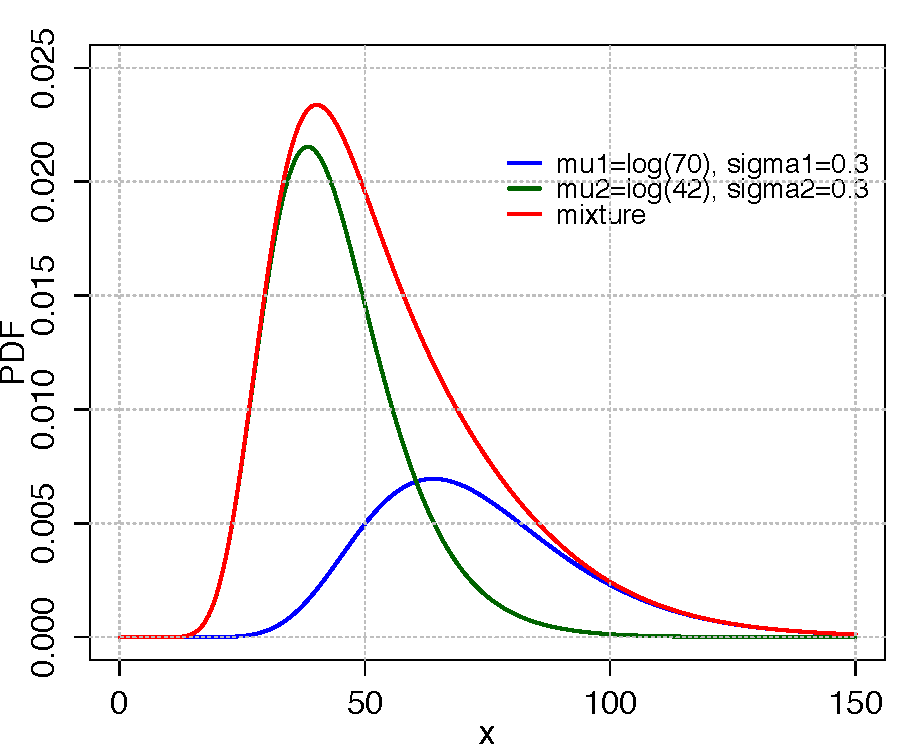
\includegraphics[width=70mm]{pics/MixtureLogNormal1.pdf}
 \caption[PDF of the Mixture of Log-Normal distribution]{PDF plot of the mixture of Log-Normal distribution.}
 \label{fig:MixtureLogNormal}
\end{figure}

It can implemented using the \xelem{MixtureDistribution} from ProbOnto
as the following code snippet shows. 

\lstset{language=XML}
\begin{lstlisting}
    <IndividualParameter symbId="V">
        <Distribution>
            <po:ProbOnto name="MixtureDistribution">
                <po:Parameter name="weight">
                    <ct:Assign>
                        <ct:SymbRef symbIdRef="pi"/>
                    </ct:Assign>
                </po:Parameter>
                <po:MixtureComponent name="LogNormal1">
                    <po:Parameter name="meanLog">
                        <ct:Assign>
                            <math:Uniop op="log">
                                <ct:SymbRef symbIdRef="mu1"/>
                            </math:Uniop>
                        </ct:Assign>
                    </po:Parameter>
                    <po:Parameter name="stdevLog">
                        <ct:Assign>
                            <ct:SymbRef symbIdRef="sigma1"/>
                        </ct:Assign>
                    </po:Parameter>
                </po:MixtureComponent>
                <po:MixtureComponent name="LogNormal1">
                    <po:Parameter name="meanLog">
                        <ct:Assign>
                            <math:Uniop op="log">
                                <ct:SymbRef symbIdRef="mu2"/>
                            </math:Uniop>
                        </ct:Assign>
                    </po:Parameter>
                    <po:Parameter name="stdevLog">
                        <ct:Assign>
                            <ct:SymbRef symbIdRef="sigma2"/>
                        </ct:Assign>
                    </po:Parameter>
                </po:MixtureComponent>
            </po:ProbOnto>
        </Distribution>
    </IndividualParameter>
\end{lstlisting}


\subsection{Mixtures of structural models}
\label{sec:mixStructModels}

All mixtures of structural models are encodable using 
the following new elements
\begin{itemize}
\item 
\xelem{MixtureModel} with 
\begin{itemize}
\item 
\xelem{StructuralModels} element which applies in all models
along with one of the following elements, dependent on the model type
\begin{itemize}
\item 
\xelem{Proportions} for WSMM
\item 
\xelem{GroupLabel} for supervised BSMM
\item 
\xelem{GroupProbabilities} for unsupervised BSMM
\end{itemize}
\item
attributes 
\begin{itemize}
\item 
\xatt{symbId} -- Id assigned to the mixture model and used later in the 
actual observation model
\item 
\xatt{type} with values \textit{wsmm}, \textit{bsmmSupervised} and \textit{bsmmUnsupervised}
\end{itemize}\end{itemize}
\end{itemize}


\subsubsection{WSMM}
\label{subsec:wsmm}
The between-subject model mixtures reads
\begin{align}
f &= \sum^M_{m=1} \pi_{m,i} f_m, \quad \sum \pi_{m,i} = 1	\nonumber
\end{align}
and it assumes inter-individual variabilities for the proportions 
of each model, $\pi_{m,i}$. Its implementation in PharmML happens 
in the \xelem{ObservationModel} element 

%between-subjects model mixtures -- each subject belongs to one sub-population 
%- supervised
%- unsupervised
\lstset{language=XML}
\begin{lstlisting}
         <ObservationModel blkId="wsmm">
            <ContinuousData>
                <PopulationParameter symbId="a"/>
                <RandomVariable symbId="eps">
                    <Distribution>
                        <po:ProbOnto name="StandardNormal1"/>
                    </Distribution>
                </RandomVariable>
                
                <MixtureModel symbId="f" type="wsmm">
                    <StructuralModels>
                        <Model>
                            <ct:Assign>
                                <ct:SymbRef blkIdRef="sm1" symbIdRef="f1"/>
                            </ct:Assign>
                        </Model>
                        <!-- omitted f2 & f3 -->
                    </StructuralModels>
                    <Proportions>
                        <Proportion>
                            <ct:Assign>
                                <ct:SymbRef blkIdRef="pm1" symbIdRef="pi1"/>
                            </ct:Assign>
                        </Proportion>
                        <!-- omitted pi2 & pi3 -->
                    </Proportions>
                </MixtureModel>
\end{lstlisting}
and $f$ can now be used to define the observation model, here one with 
a constant error model
\lstset{language=XML}
\begin{lstlisting}
                <Standard symbId="Yobs">
                    <Transformation type="identity"/>
                    <Output>
                        <ct:SymbRef symbIdRef="f"/>
                    </Output>
                    <ErrorModel>
                        <ct:Assign>
                            <ct:SymbRef symbIdRef="a"/>
                        </ct:Assign>
                    </ErrorModel>
                    <ResidualError>
                        <ct:SymbRef symbIdRef="eps"/>
                    </ResidualError>
                </Standard>
                
            </ContinuousData>
        </ObservationModel>
\end{lstlisting}



\subsubsection{BSMM}
\label{subsec:bsmm}

\begin{align}
f &= \sum^M_{m=1} \mathbbm{1}_{m=z} f_m	\nonumber
\end{align}


\subsubsection*{Supervised}
In this case, the group membership is known and the regressor
variable $z$ is used to identify it. E.g. in MLXTRAN it is used to condition 
on and to select the appropriate structural model as the following 
code snippet shows:
\lstset{language=MLX}
\begin{lstlisting}
		g = {use=regressor}
		EQUATION:
		if g==1
   			f = A1
		else
   			f = A2*exp(-k*max(t,0))
		end
\end{lstlisting}
while in PharmML the previously introduced elements are used

\lstset{language=XML}
\begin{lstlisting}
        <ObservationModel blkId="bsmm">
            <ContinuousData>
                <PopulationParameter symbId="a"/>
                <ct:Variable symbId="z" regressor="yes"/>
                
                <RandomVariable symbId="eps">
                    <Distribution>
                        <po:ProbOnto name="StandardNormal1"/>
                    </Distribution>
                </RandomVariable>
                
                <MixtureModel symbId="f" type="bsmmSupervised">
                    <StructuralModels>
                        <Model>
                            <ct:Assign>
                                <ct:SymbRef blkIdRef="sm1" symbIdRef="f1"/>
                            </ct:Assign>
                        </Model>
                        <!-- omitted F2 -->
                        <Model>
                            <ct:Assign>
                                <ct:SymbRef blkIdRef="sm1" symbIdRef="f3"/>
                            </ct:Assign>
                        </Model>
                    </StructuralModels>
                    <GroupLabel>
                        <ct:Assign>
                            <ct:SymbRef symbIdRef="z"/>
                        </ct:Assign>
                    </GroupLabel>
                </MixtureModel>
                
                <Standard symbId="Yobs">
                        <!-- omitted for brevity -->
                </Standard>
                
            </ContinuousData>
        </ObservationModel>

\end{lstlisting}


\subsubsection*{Unsupervised}
In this case, the group membership is not known and its proportion, expressed
by the population parameter $p$, in the population is to be estimated. 

\bigskip
MLXTRAN code for this model reads:
\lstset{language=MLX}
\begin{lstlisting}
		EQUATION:
		f1 = A1
		f2 = A2*exp(-k*max(t,0))
		f=bsmm(f1, p, f2, 1-p)
\end{lstlisting}

The following PharmML implementation handles the BSMM model only, 
the implementation of the structural models $f_1$ and $f_2$, encoded in 
\xelem{StructuralModel} \xatt{sm1}, are not shown.

\lstset{language=XML}
\begin{lstlisting}
        <ObservationModel blkId="bsmm2">
            <ContinuousData>
                <PopulationParameter symbId="a"/>
                <RandomVariable symbId="eps">
                    <Distribution>
                        <po:ProbOnto name="StandardNormal1"/>
                    </Distribution>
                </RandomVariable>
                
                <MixtureModel symbId="f" type="bsmmUnsupervised">
                    <StructuralModels>
                        <Model>
                            <ct:Assign>
                                <ct:SymbRef blkIdRef="sm1" symbIdRef="f1"/>
                            </ct:Assign>
                        </Model>
                        <Model>
                            <ct:Assign>
                                <ct:SymbRef blkIdRef="sm1" symbIdRef="f2"/>
                            </ct:Assign>
                        </Model>
                    </StructuralModels>
                    <GroupProbabilities>
                        <GroupProbability>
                            <ct:Assign>
                                <ct:SymbRef blkIdRef="pm1" symbIdRef="p"/>
                            </ct:Assign>
                        </GroupProbability>
                        <GroupProbability>
                            <ct:Assign>
                                <math:Binop op="minus">
                                    <ct:Real>1</ct:Real>
                                    <ct:SymbRef blkIdRef="pm1" symbIdRef="p"/>
                                </math:Binop>
                            </ct:Assign>
                        </GroupProbability>
                    </GroupProbabilities>
                </MixtureModel>
                             
                <Standard symbId="Yobs">
                    <!-- Yobs = f + a*eps; omitted for brevity -->
                </Standard>
                
            </ContinuousData>
        </ObservationModel>
\end{lstlisting}


%%%%%%%%%%%%%%%%%%%%%%%%%%%%%
\subsection{SymbRef assignments extensions}
\label{subsec:symbRefAssign}
In a number of cases \xelem{SymbRef} was the only assignment option.
This obviously restrictive structure has been extended to a general assignment
using \xelem{Assign} allowing for virtually any expression. Elements where
the new possibility is present are e.g.  
\begin{itemize}
\item 
\xelem{RandomVariable1}, \xelem{RandomVariable2} -- used in the correlation
of random effects element
\item
\xelem{FixedEffect} -- assignment of fixed effects in structured parameter 
model
\item
\xelem{RandomEffect}  -- assignment of random effects in structured parameter.
\end{itemize}

%\subsection{Assignments allowed}
%\label{subsec:assign}
\paragraph{Example 1}
Element \xelem{RandomEffects} accept now any assignment, e.g. sum
of two fixed effects
\lstset{language=XML}
\begin{lstlisting}
                    <FixedEffect>
                        <ct:Assign>
                            <math:Binop op="plus">
                                <ct:SymbRef blkIdRef="pm" symbIdRef="BETA_WT"/>
                                <ct:SymbRef blkIdRef="pm" symbIdRef="BETA_CL"/>
                            </math:Binop>
                        </ct:Assign>
                    </FixedEffect>
\end{lstlisting}

\paragraph{Example 2}
It is possible to assign a specific vector/matrix element to \xelem{RandomEffects}, e.g.
\lstset{language=XML}
\begin{lstlisting}
                    <RandomEffects>
                        <ct:Assign>
                            <ct:VectorSelector>
                                <ct:SymbRef blkIdRef="pm" symbIdRef="ETA_CL_V_KA"/>
                                <ct:Cell>
                                    <ct:Assign>
                                        <ct:Int>1</ct:Int>
                                    </ct:Assign>
                                </ct:Cell>
                            </ct:VectorSelector>
                        </ct:Assign>
                    </RandomEffects>
\end{lstlisting}

%%%%%%%%%%%%%%%%%%%%%%%%%%%%%%%%%%%%%%%%%%%%%%%%%%%%%%%%%%%%%%%%%%%%%%
\section{Covariate model}
\label{sec:covModel}

\subsection{Fixing a bug in referencing of covariate categories}
\label{subsec:fixingRefs}
A defined categorical covariate, e.g.   sex with two categories $F$ and $M$
\lstset{language=XML}
\begin{lstlisting}
        <CovariateModel blkId="cm1">
            <Covariate symbId="Sex">
                <Categorical>
                    <Category catId="F"/>
                    <Category catId="M"/>
                </Categorical>
            </Covariate>
        </CovariateModel>
\end{lstlisting}
is usually used in the parameter model, \xelem{StructuredModel}, i.e. 
within the \xelem{FixedEffect} element as shown in Table \ref{tab:catCovRefs} (left).
The use of the \xelem{Category} however is inconsistent as it was designed
to define new categories via the \xatt{catId} attribute rather then to refer to 
existing ones as in this case.

Therefore, when refering to an existing categories, one should use the \xelem{CatRef}
element, see Table \ref{tab:catCovRefs} (right).

\begin{longtable}{cc}
\hline
\hline
support in $\le$ 0.8.1 & support in v0.9 \\
\hline
\lstset{language=XML}
\begin{lstlisting}
<IndividualParameter symbId="V">
    <StructuredModel>
        <Transformation type="log"/>
        <LinearCovariate>
                ...
            <Covariate>
                <ct:SymbRef symbIdRef="Sex"/>
                <FixedEffect>
                    <ct:SymbRef symbIdRef="beta_V"/>
                    <Category catId="F"/>
                </FixedEffect>
            </Covariate>
        </LinearCovariate>
            ...
    </StructuredModel>
</IndividualParameter>
\end{lstlisting}
&
\lstset{language=XML}
\begin{lstlisting}
<IndividualParameter symbId="V">
    <StructuredModel>
        <Transformation type="log"/>
        <LinearCovariate>
                ...
            <Covariate>
                <ct:SymbRef symbIdRef="Sex"/>
                <FixedEffect>
                    <ct:SymbRef symbIdRef="beta_V"/>
                    <ct:CatRef catIdRef="F"/>
                </FixedEffect>
            </Covariate>
        </LinearCovariate>
            ...
    </StructuredModel>
</IndividualParameter>
\end{lstlisting}
\\
\hline
\caption{Referencing of categories of categorical covariates in structured parameter
model. Instead of \xelem{Category} with \xatt{catId} attribute, the \xelem{CatRef} 
element should be used. For brevity, the block reference \xatt{blkIdRef="cm1"} has
been removed along with \xelem {PopulationValue} and \xelem{RandomEffects} elements.}
\label{tab:catCovRefs}
\end{longtable}%



%%%%%%%%%%%%%%%%%%%%%%%%%%%%
\subsection{Categorical covariate building -- clustering}
\label{subset:catCovTrans}
Based on other existing covariates, new  categorical covariates can 
be now declared using the so called 'clustering', a mechanism allowing 
for grouping of categories to define new, more general ones.

\bigskip
New elements and extensions 
\begin{itemize}
\item 
boolean reference category, \xatt{referenceCategory}, attribute
\item
\xelem{CatRef} can be used directly to build new categories by referring to existing ones
\item
\xelem{CatRef} equipped with additional \xatt{symbIdRef} and \xatt{blkIdRef} attributes
\item
the general assignment via \xelem{Assign} is also available.
\end{itemize}


\subsubsection*{Example} Building new covariate, via clustering of categories of
a base covariate, following an MXTRAN example

\lstset{language=MLX}
\begin{lstlisting}
            VARIABLES: 
            	t_GENOTYPE = transform(
            		GENOTYPE,
            		G1 = {1} reference,
            		G2 = {2,3,4}
            		) [use=cov,  type=cat]
\end{lstlisting}
where a transformed covariate 't\_GENOTYPE' is declared based
on the 'GENOTYPE' covariate.	

\bigskip
PharmML implementation reads
\begin{itemize}
\item 
formulate the base covariate as 
\lstset{language=XML}
\begin{lstlisting}
            <Covariate symbId="GENOTYPE">        
                <Categorical>
                    <Category catId="GENOTYPE_cat_1"/>
                    <Category catId="GENOTYPE_cat_2"/>
                    <Category catId="GENOTYPE_cat_3"/>
                    <Category catId="GENOTYPE_cat_4"/>
                </Categorical>
            </Covariate>
\end{lstlisting}
\item
and declare the new one out of the categories of the \emph{GENOTYPE} covariate
\end{itemize}
\lstset{language=XML}
\begin{lstlisting}            
            <Covariate symbId="t_GENOTYPE">        
                <Categorical>
                    <Category catId="G1" referenceCategory="true">
                        <!-- blkIdRef="cm2" could be used additionally if the reference covariate was  -->
                        <!-- declared in a different covariate model, "cm2" -->
                        <ct:CatRef symbIdRef="GENOTYPE" catIdRef="GENOTYPE_cat_1"/>
                    </Category>
                    <Category catId="G2">
                        <ct:CatRef symbIdRef="GENOTYPE" catIdRef="GENOTYPE_cat_2"/>
                        <ct:CatRef symbIdRef="GENOTYPE" catIdRef="GENOTYPE_cat_3"/>
                        <ct:CatRef symbIdRef="GENOTYPE" catIdRef="GENOTYPE_cat_4"/>
                    </Category>
                </Categorical>
            </Covariate>
\end{lstlisting}
Note that we use the \xelem{ct:CatRef} element to declare a new category 
together with the \xatt{symbIdRef} attribute pointing to the reference covariate.
Additionally \xatt{blkIdRef} can be used if the reference covariate was declared 
in another covariate model.

\subsection{Latent covariates}
\label{subsec:latent}

Adding \textit{latent} to the covariate type attribute allows to declare
any number of latent categorical covariates with any number of
categories. The implementation is performed using the 
\begin{itemize}
\item 
new value, \textit{latent}, of the \xatt{type} attribute
\item 
and the \xelem{NumberOfCategories} element
\end{itemize}
as the following code snippet illustrates. We consider a case when 
the latent covariate has two categories which can be treated as population 
values to be estimated.

\lstset{language=XML}
\begin{lstlisting}
            <Covariate type="latent" symbId="lCat">
                <Categorical>
                    <Category catId="lcat1">
                        <ct:Assign>
                            <ct:SymbRef blkIdRef="pm1" symbIdRef="plcat1"/>
                        </ct:Assign>
                    </Category>
                    <Category catId="lcat2">
                        <ct:Assign>
                            <ct:SymbRef blkIdRef="pm1" symbIdRef="plcat2"/>
                        </ct:Assign>
                    </Category>
                    <NumberOfCategories>
                        <ct:Assign>
                            <ct:Real>2</ct:Real>
                        </ct:Assign>
                    </NumberOfCategories>
                </Categorical>
            </Covariate>
\end{lstlisting}
Note that e.g. Monolix has a naming convention for latent covariates 
and their categories in which case the specification of the number of 
categories for such covariate only is sufficient. 



\subsection{Covariate exclusion \& inclusion criteria}
\label{subsec:exclInclCriteria}
This version comes with another extension in handling of 
covariates, i.e. possibility to declare (any number of)
\begin{itemize}
\item 
exclusion and/or
\item
inclusion
\end{itemize}
criteria on continous covariates, e.g. inclusion of subject with BMI
between 20 and 25
\lstset{language=XML}
\begin{lstlisting}
            <Covariate symbId="BMI">
                <Continuous>
                    <Criteria type="inclusive">
                        <math:LogicBinop op="and">
                            <math:LogicBinop op="geq">
                                <ct:SymbRef symbIdRef="BMI"/>
                                <ct:Real>20</ct:Real>
                            </math:LogicBinop>
                            <math:LogicBinop op="leq">
                                <ct:SymbRef symbIdRef="BMI"/>
                                <ct:Real>25</ct:Real>
                            </math:LogicBinop>
                        </math:LogicBinop>
                    </Criteria>
                </Continuous>
            </Covariate>
\end{lstlisting}
and categorical covariates, e.g. exclusion of female subjects
\lstset{language=XML}
\begin{lstlisting}
            <Covariate symbId="Sex">
                <Categorical>
                    <Category catId="F"/>
                    <Category catId="M"/>
                    <Criteria type="exclusive">
                        <math:LogicBinop op="eq">
                            <ct:SymbRef symbIdRef="Sex"/>
                            <ct:CatRef catIdRef="F"/>
                        </math:LogicBinop>
                    </Criteria>
                </Categorical>
            </Covariate>
\end{lstlisting}
as the code snippets illustrate. They can be applied in all types of tasks 
but might be especially of interest in simulation and optimal design oriented models.


%%%%%%%%%%%%%%%%%%%%%%%%%%%%%%%%%%%%%%%%%%%%%%%%%%%%%%%%%%%%%%%%%%%%%%
\section{Parameter model}
\label{sec:paramModel}

\subsection{Correlation of random effects/parameters}

Consider a model with following parameters
\begin{align}
\log(a) &\sim \mathcal{N}(\log(a_{pop}), \omega_a^2) \nonumber \\
b &\sim \mathcal{N}(b_{pop}), \omega_b^2) \nonumber \\
\mbox{logit}(c) &\sim \mathcal{N}(\mbox{logit}(c_{pop}), \omega_c^2) \nonumber 
\end{align}
with correlation matrix for the vector ($\log(a)$, $b$, $\text{logit}(c)$) which reads
\begin{align}
R = 
\begin{bmatrix} 1 & r_{ab} & r_{bc}  \\
 r_{bc} &  1 & r_{bc} \\
 r_{bc} & r_{bc} & 1 \nonumber
 \end{bmatrix}
\end{align}
\smallskip
There are two new ways to encode the above correlation structure
\begin{itemize}
\item 
Option 1: Pairwise correlation for transformed parameters, here one
pair is shown only 
\begin{align}
corr(\log(a), \text{logit}(c)) = r_{ac}\nonumber 
\end{align}
reads in PharmML
\lstset{language=XML}
\begin{lstlisting}
            <Correlation>
                <ct:VariabilityReference>
                    <ct:SymbRef blkIdRef="vm1" symbIdRef="indiv"/>
                </ct:VariabilityReference>
                <Pairwise>
                    <RandomVariable1>
                        <ct:Assign>
                            <math:Uniop op="log">
                                <ct:SymbRef symbIdRef="a"/>
                            </math:Uniop>                            
                        </ct:Assign>
                    </RandomVariable1>
                    <RandomVariable2>
                        <ct:Assign>
                            <math:Uniop op="log">
                                <ct:SymbRef symbIdRef="c"/>
                            </math:Uniop>                            
                        </ct:Assign>
                    </RandomVariable2>
                    <CorrelationCoefficient>
                        <ct:Assign>
                            <ct:SymbRef symbIdRef="r_ac"/>
                        </ct:Assign>
                    </CorrelationCoefficient>
                </Pairwise>
            </Correlation>
\end{lstlisting}
\item 
Option 2: Matrix correlation, R, for entire parameter vector
\begin{align}
(\log(a), b, \text{logit}(c))\nonumber 
\end{align}
using the \xelem{Correlation} element notation extended with the 
\begin{itemize}
\item 
standard \xelem{Assign} element, preceding the \xelem{Matrix} and 
\xelem{Pairwise} elements, to encode the parameter vector 
capable to hold any combination of transformed or untransformed 
parameters
\end{itemize}
as the following code snippet demonstrates
 
\lstset{language=XML}
\begin{lstlisting}
            <Correlation deviationMatrixType="CorrMatrix">
                <ct:VariabilityReference>
                    <ct:SymbRef blkIdRef="vm1" symbIdRef="indiv"/>
                </ct:VariabilityReference>
                <ct:Assign>
                    <ct:Vector>
                        <ct:VectorElements>
                            <ct:Assign>
                                <math:Uniop op="log">
                                    <ct:SymbRef symbIdRef="a"/>
                                </math:Uniop>
                            </ct:Assign>
                            <ct:Assign>
                                <ct:SymbRef symbIdRef="b"/>
                            </ct:Assign>
                            <ct:Assign>
                                <math:Uniop op="logit">
                                    <ct:SymbRef symbIdRef="c"/>
                                </math:Uniop>
                            </ct:Assign>
                        </ct:VectorElements>
                    </ct:Vector>
                </ct:Assign>
                <Matrix matrixType="Symmetric">
                    <ct:MatrixRow>
                        <ct:Real>1</ct:Real>
                    </ct:MatrixRow>
                    <ct:MatrixRow>
                        <ct:SymbRef symbIdRef="r_ab"/><ct:Real>1</ct:Real>
                    </ct:MatrixRow>
                    <ct:MatrixRow>
                        <ct:SymbRef symbIdRef="r_ac"/><ct:SymbRef symbIdRef="r_bc"/><ct:Real>1</ct:Real>
                    </ct:MatrixRow>
                </Matrix>
            </Correlation>
\end{lstlisting}

\end{itemize}



%%%%%%%%%%%%%%%%%%%%%%%%%%%%%%%%%%%%%%%%%%%%%%%%%%%%%%%%%%%%%%%%%%%%%%
\section{Observation model}
\label{sec:obsModel}
\subsection{Multiple models allowed per block}

Consider continuous PK/PD model implemented as "example1\_NONMEM.xml" 
in the release pack. Instead of declaring separate blocks, the PK and PD models 
can be now combined within one \xelem{ObservationModel}. 
Note, that the data mapping needs to be accordingly amended and parameter $a$, 
used in both models, has been duplicated as $a1$ and $a2$.


\begin{align}
E_{obs} &= E + a_1 \;\epsilon_{E} \nonumber \\
Cc_{obs} &= Cc + (a_2 + b\;Cc) \;\epsilon_{Cc}  \nonumber
\end{align}


\lstset{language=XML}
\begin{lstlisting}
        <ObservationModel blkId="om1">
            <ContinuousData>
                <PopulationParameter symbId="a1"/>
                <PopulationParameter symbId="a2"/>
                <PopulationParameter symbId="b"/>

                <RandomVariable symbId="epsilon_Cc">
                    <!-- omitted details -->
                </RandomVariable>
                <RandomVariable symbId="epsilon_E">
                    <!-- omitted details -->
                </RandomVariable>
                
                <!-- FIRST MODEL -->
                <General symbId="E_obs">
                    <ct:Assign>
                        <math:Binop op="plus">
                            <ct:SymbRef blkIdRef="sm1" symbIdRef="E"/>
                            <math:Binop op="times">
                                <math:FunctionCall>
                                    <ct:SymbRef symbIdRef="constantErrorModel"/>
                                    <!-- omitted arguments -->
                                </math:FunctionCall>
                                <ct:SymbRef symbIdRef="epsilon_E"/>
                            </math:Binop>
                        </math:Binop>
                    </ct:Assign>
                </General>

                <!-- SECOND MODEL - this was not allowed previously -->
                <Standard symbId="Cc_obs">
                    <Output>
                        <ct:SymbRef blkIdRef="sm1" symbIdRef="Cc"/>
                    </Output>
                    <ErrorModel>
                        <ct:Assign>
                            <math:FunctionCall>
                                <ct:SymbRef symbIdRef="combinedErrorModel"/>
                                <!-- omitted arguments -->
                            </math:FunctionCall>
                        </ct:Assign>
                    </ErrorModel>
                    <ResidualError>
                        <ct:SymbRef symbIdRef="epsilon_Cc"/>
                    </ResidualError>
                </Standard>
                
            </ContinuousData>
        </ObservationModel>
\end{lstlisting}

\subsection{Models are allowed in conditionals}

\subsubsection*{Example 1}
Different model types dependent on FLAG value can be declared, e.g.

\begin{eqnarray}
&& \left\{ \begin{array}{lcl}  Cc_{obs} = Cc + a_1 \;\epsilon_{Cc}  & \mbox{for} & \mbox{FLAG}  == 1	 \\
Cc_{obs} = Cc + (a_2 + b\;Cc) \;\epsilon_{E} & \mbox{for} & \mbox{FLAG} == 2 \nonumber
\end{array}\right.
\end{eqnarray}


\lstset{language=XML}
\begin{lstlisting}
        <ObservationModel blkId="om2">
            <ContinuousData>
                <PopulationParameter symbId="a1"/>
                <PopulationParameter symbId="a2"/>
                <PopulationParameter symbId="b"/>
                
                <ct:Variable regressor="yes" symbId="FLAG"/>

                <RandomVariable symbId="epsilon_Cc">
                    <!-- omitted -->
                </RandomVariable>
                <RandomVariable symbId="epsilon_E">
                    <!-- omitted -->
                </RandomVariable>
                
                <ct:Variable symbId="Cc_obs"/>
                
                <math:ConditionalStatement>
                    <!-- FIRST CONDITION -->
                    <math:If>
                        <math:Condition>
                            <math:LogicBinop op="eq">
                                <ct:SymbRef symbIdRef="FLAG"/>
                                <ct:Real>1</ct:Real>
                            </math:LogicBinop>
                        </math:Condition>
                        <General symbIdRef="Cc_obs">
                            <ct:Assign>
                                <math:Binop op="plus">
                                    <ct:SymbRef blkIdRef="sm1" symbIdRef="Cc"/>
                                    <math:Binop op="times">
                                        <math:FunctionCall>
                                            <ct:SymbRef symbIdRef="constantErrorModel"/>
                                            <!-- omitted arguments -->
                                        </math:FunctionCall>
                                        <ct:SymbRef symbIdRef="epsilon_Cc"/>
                                    </math:Binop>
                                </math:Binop>
                            </ct:Assign>
                        </General>
                    </math:If>
                    <!-- SECOND CONDITION -->
                    <math:ElseIf>
                        <math:Condition>
                            <math:LogicBinop op="eq">
                                <ct:SymbRef symbIdRef="FLAG"/>
                                <ct:Real>2</ct:Real>
                            </math:LogicBinop>
                        </math:Condition>
                        <Standard symbIdRef="Cc_obs">
                            <Output>
                                <ct:SymbRef blkIdRef="sm1" symbIdRef="Cc"/>
                            </Output>
                            <ErrorModel>
                                <ct:Assign>
                                    <math:FunctionCall>
                                        <ct:SymbRef symbIdRef="combinedErrorModel"/>
                                        <!-- omitted arguments -->
                                    </math:FunctionCall>
                                </ct:Assign>
                            </ErrorModel>
                            <ResidualError>
                                <ct:SymbRef symbIdRef="epsilon_Cc"/>
                            </ResidualError>
                        </Standard>
                    </math:ElseIf>
                </math:ConditionalStatement>
                
            </ContinuousData>
        </ObservationModel>
\end{lstlisting}


\subsubsection*{Example 2}

An alternative version of the previous model with a 
\begin{itemize}
\item 
structured and 
\item 
distribution 
\end{itemize}
based models, dependent on FLAG value, respectively.

\begin{eqnarray}
&& \left\{ \begin{array}{lcl}  Cc_{obs} = Cc + a \;\epsilon_{Cc}  & \mbox{for} & \mbox{FLAG}  == 1	 \\
Cc_{obs} \sim \mathcal{N}\big(Cc, (a + b\;Cc)\big) & \mbox{for} & \mbox{FLAG} == 2 \nonumber
\end{array}\right.
\end{eqnarray}


\lstset{language=XML}
\begin{lstlisting}
        <ObservationModel blkId="om3">
            <ContinuousData>
                <PopulationParameter symbId="a1"/>
                <PopulationParameter symbId="a2"/>
                <PopulationParameter symbId="b"/>
                
                <ct:Variable regressor="yes" symbId="FLAG"/>

                <RandomVariable symbId="epsilon_Cc">
                    <!-- omitted -->
                </RandomVariable>
                
                <ct:Variable symbId="Cc_obs"/>
                
                <math:ConditionalStatement>
                    <math:If>
                        <math:Condition>
                            <math:LogicBinop op="eq">
                                <ct:SymbRef symbIdRef="FLAG"/>
                                <ct:Real>1</ct:Real>
                            </math:LogicBinop>
                        </math:Condition>
                        <General symbIdRef="Cc_obs">
                            <ct:Assign>
                                <math:Binop op="plus">
                                    <ct:SymbRef blkIdRef="sm1" symbIdRef="Cc"/>
                                    <math:Binop op="times">
                                        <math:FunctionCall>
                                            <ct:SymbRef symbIdRef="constantErrorModel"/>
                                            <!-- omitted arguments -->
                                        </math:FunctionCall>
                                        <ct:SymbRef symbIdRef="epsilon_Cc"/>
                                    </math:Binop>
                                </math:Binop>
                            </ct:Assign>
                        </General>
                    </math:If>
                    <math:ElseIf>
                        <math:Condition>
                            <math:LogicBinop op="eq">
                                <ct:SymbRef symbIdRef="FLAG"/>
                                <ct:Real>2</ct:Real>
                            </math:LogicBinop>
                        </math:Condition>
                        <General symbIdRef="Cc_obs">
                            <Distribution>
                                <po:ProbOnto name="Normal1">
                                    <po:Parameter name="mean">
                                        <ct:Assign>
                                            <ct:SymbRef blkIdRef="sm1" symbIdRef="Cc"/>
                                        </ct:Assign>
                                    </po:Parameter>
                                    <po:Parameter name="stdev">
                                        <ct:Assign>
                                            <math:Binop op="plus">
                                                <ct:SymbRef symbIdRef="a2"/>
                                                <math:Binop op="times">
                                                    <ct:SymbRef symbIdRef="b"/>
                                                    <ct:SymbRef blkIdRef="sm1" symbIdRef="Cc"/>
                                                </math:Binop>
                                            </math:Binop>
                                        </ct:Assign>
                                    </po:Parameter>
                                </po:ProbOnto>
                            </Distribution>
                        </General>
                    </math:ElseIf>
                </math:ConditionalStatement>
                
            </ContinuousData>
        </ObservationModel>
\end{lstlisting}


\subsection{Missing element restored}
During the refactoring/extension of the observation model in version 0.7-0.7.2
we have lost the left-hand side transformation, $h$ in the formula below, 
option for the \xelem{General} model, \cite{Pharmml_06}.
\begin{align}
 h(y) = H(...) \nonumber
\end{align}
Models like that below, \cite{Beal:2001}, were still encodable but using the distribution-type
notation or the very generic \xelem{AssignStatement} element, as shown below.

\bigskip
Model definition:
\begin{eqnarray}
\log(y_{ij}) =  \log(f_{ij}+M) + \frac{f_{ij}}{f_{ij}+M} \epsilon_{1,ij} + \frac{M}{f_{ij}+M} \epsilon_{2,ij}; \quad \mathit{var}(y_{ij}) = \frac{f_{ij}^2 + M^2}{(f_{ij}+M)^2} \label{eq:beal2001_1}
\end{eqnarray}
for uncorrelated $\epsilon_{1,ij}, \epsilon_{2,ij}\sim N(0,1)$ .
\bigskip

\begin{eqnarray}
 \log(y_{ij}) \sim \mathcal{N}\Big( \log(f_{ij}+M), \frac{f_{ij}^2 + M^2}{(f_{ij}+M)^2} \Big) \label{eq:beal2001_2}
\end{eqnarray}
Model (\ref{eq:beal2001_1}) reads in PharmML

\lstset{language=XML}
\begin{lstlisting}
    <ObservationModel blkId="Beal2001">
        <ContinuousData>
            <PopulationParameter symbId="M"/>
            <ct:Variable symbId="y"/>
            
            <RandomVariable symbId="eps1">
                <Distribution>
                    <po:ProbOnto name="StandardNormal1"/>
                </Distribution>
            </RandomVariable>
            <RandomVariable symbId="eps2">
                <Distribution>
                    <po:ProbOnto name="StandardNormal1"/>
                </Distribution>
            </RandomVariable>
            
            <ct:AssignStatement op="eq">
                <math:Uniop op="log">
                    <ct:SymbRef symbIdRef="y"/>
                </math:Uniop>
                <math:Binop op="plus">
                    <math:Uniop op="log">
                        <math:Binop op="plus">
                            <ct:SymbRef blkIdRef="sm1" symbIdRef="f"/>
                            <ct:SymbRef symbIdRef="M"/>
                        </math:Binop>
                    </math:Uniop>
                    <math:Binop op="plus">
                        <!-- () * eps1 -->
                        <math:Binop op="times">
                            <math:Binop op="divide">
                                <ct:SymbRef blkIdRef="sm1" symbIdRef="f"/>
                                <math:Binop op="plus">
                                    <ct:SymbRef blkIdRef="sm1" symbIdRef="f"/>
                                    <ct:SymbRef symbIdRef="M"/>
                                </math:Binop>
                            </math:Binop>
                            <ct:SymbRef symbIdRef="eps1"/>
                        </math:Binop>
                        <!-- () * eps2 -->
                        <math:Binop op="times">
                            <math:Binop op="divide">
                                <ct:SymbRef symbIdRef="M"/>
                                <math:Binop op="plus">
                                    <ct:SymbRef blkIdRef="sm1" symbIdRef="f"/>
                                    <ct:SymbRef symbIdRef="M"/>
                                </math:Binop>
                            </math:Binop>
                            <ct:SymbRef symbIdRef="eps2"/>
                        </math:Binop>
                    </math:Binop>
                </math:Binop>
            </ct:AssignStatement>
        </ContinuousData>
    </ObservationModel>
\end{lstlisting}

Model (\ref{eq:beal2001_2}) is not shown but is straightforward to 
implement using the D-Type parameter model.


%%%%%%%%%%%%%%%%%%%%%%%%%%%%
\subsection{Removed redundant named parameters}
\label{subsec:namedParams}

Following, redundant, named parameters element have been removed
from the observation model for count data: \xelem{IntensityParameter}, 
\xelem{DispersionParameter}, \xelem{OverDispersionParameter}, 
\xelem{ZeroProbabilityParameter}, \xelem{MixtureProbabilityParameter}.



%%%%%%%%%%%%%%%%%%%%%%%%%%%%%%%%%%%%%%%%%%%%%%%%%%%%%%%%%%%%%%%%%%%%%%
\section{Autocorrelation of residual errors}
\label{subsec:autoCorr}
Although nearly from the very beginning on the to-do list,  support 
of the autocorrelation of residual errors, is only now available and it comes in 
many different flavours. 
A discussion of correlation models, based on which the following support has been
designed, can be found in \cite{DavidianLecture:2009}, 
\cite{Bonate:2011fk} or \cite{LavielleBook:2014}.

\bigskip
We distinguish between the following correlation models 
\begin{itemize}
\item
independent
\item
unstructured
\item
exchangeable/compound symmetric
\item
one-dependent
\item
two-dependent
\item
auto-regressive AR(1)
\item
exponential
\item
gaussian
\end{itemize}
%Note, that on every model type is useful for a particular problem. Davidian argues that 

%%%%%%%%%%%%%%%%%%%%%%%%%%%%%%
\subsection{General models}
In the following, the index $i$ is used to indicate subject, $j$ to indicate the time point.

%%%%%%%%%%%%%%%%%%%%%%%%%%%%%%
\subsection*{Independent model}
The correlation matrix of the simplest model reads
\[
 \Gamma_i =
 \begin{pmatrix}
  	1 		& 0		 	& 0 			& \cdots 		& 0 \\
	0		& 1 			& 0		 	& \cdots 		& 0 \\
	0		& 0			& 1 			& \cdots 		& 0 \\
	\vdots 	& \vdots		& \vdots		& \ddots		& \vdots \\
	0		& \cdots		& 0			& 0			& 1 	
 \end{pmatrix}
\]


%%%%%%%%%%%%%%%%%%%%%%%%%%%%%%
\subsection*{Unstructured model}
The correlation matrix of this most general model reads
\[
 \Gamma_i(\alpha) =
 \begin{pmatrix}
  1 			& \alpha_{12}  	& \alpha_{13} 	& \cdots 	& \alpha_{1n_i} \\
\alpha_{21}	& 1  			& \alpha_{23} 	& \cdots 	& \alpha_{2n_i} \\
\alpha_{31}	& \alpha_{32}	& 1 			& \cdots 	& \alpha_{3n_i} \\
\cdots		& \cdots		& \cdots		& \ddots	& \vdots \\
\alpha_{n_i 1}	& \alpha_{n_i 2}& \alpha_{n_i3}& \alpha_{n_i,n_{i-1}}	& 	1
 \end{pmatrix}, \quad 0 \le \alpha_{jj'} \le 1
\]
with $\alpha_{j,j'} = \alpha_{j',j}$. This model is also called \textit{unstructured} 
as there is no mathematical relation between the level of correlation and index 
of the time course. In other words, all correlations are uncommon and unique 
to each subject.

%%%%%%%%%%%%%%%%%%%%%%%%%%%%%%
\subsection*{Exchangeable/compound symmetric model}
The correlation matrix reads
\[
 \Gamma_i(\alpha) =
 \begin{pmatrix}
  1 		& \alpha 	& \alpha 	& \cdots & \alpha \\
\alpha	& 1 		& \alpha	& \cdots & \alpha \\
\alpha	& \alpha 	& 1		& \cdots & \alpha \\
\vdots	& \vdots	& \vdots	& \ddots & \vdots \\
\alpha	& \alpha	& \alpha 	& \cdots &1
 \end{pmatrix}
\]
This model assumes constant correlation between measurements.

%%%%%%%%%%%%%%%%%%%%%%%%%%%%%%
\subsection{Standard time series models}

%%%%%%%%%%%%%%%%%%%%%%%%%%%%%%
\subsection*{One-dependent model}

The correlation matrix reads
\[
 \Gamma_i(\alpha) =
 \begin{pmatrix}
  	1 		& \alpha_1 	& 0 			& \cdots 		& 0 \\
	\alpha_1	& 1 			& \alpha_2 	& \cdots 		& 0 \\
	0		& \alpha_2	& 1 			& \cdots 		& 0 \\
	\vdots 	& \vdots		& \vdots		& \ddots		& \vdots \\
	0		& \cdots		& 0			& \alpha_{n_i-1}	& 1 	
 \end{pmatrix}
\]
A special case of this model arises if one assumes that $\alpha_j \equiv \alpha$
\[
 \Gamma_i(\alpha) =
 \begin{pmatrix}
  	1 		& \alpha	 	& 0 			& \cdots 		& 0 \\
	\alpha	& 1 			& \alpha	 	& \cdots 		& 0 \\
	0		& \alpha		& 1 			& \cdots 		& 0 \\
	\vdots 	& \vdots		& \vdots		& \ddots		& \vdots \\
	0		& \cdots		& 0			& \alpha		& 1 	
 \end{pmatrix}
\]
This model assumes that each observation is correlated with the nearest neighbour only.

%%%%%%%%%%%%%%%%%%%%%%%%%%%%%%
\subsection*{Two-dependent model}

\cite{Bonate:2011fk} describes a model which assumes correlation with two neighbour time points
and its matrix reads
\[
 \Gamma_i(\alpha) =
 \begin{pmatrix}
  	1 		& \alpha_1 	& \alpha_2 	& 0 			& \cdots 		& 0 \\
	\alpha_1	& 1 			& \alpha_1 	& \alpha_2	& \cdots 		& 0 \\
	\alpha_2	& \alpha_1	& 1 			& \alpha_1 	& \cdots		& 0 \\
	0		& \alpha_2	& \alpha_1	& 1 			& \cdots 		& 0 \\
	\vdots 	& \vdots		& \vdots		& \vdots		& \ddots		& \vdots \\
	0		& \cdots		& \alpha_2	& \alpha_1	& 1			& \alpha_1 	\\
	0		& \cdots		& 0			& \alpha_2	& \alpha_1	& 1 	
 \end{pmatrix}
\]


%%%%%%%%%%%%%%%%%%%%%%%%%%%%%%
\subsection*{Autoregressive model of order 1, AR(1)}
This model holds under a number of assumptions, such as equidistant time steps. (For more details see e.g. https://onlinecourses.science.psu.edu/stat510/?q=node/60)
\[
 \Gamma_i(\alpha) =
 \begin{pmatrix}
 1 			& \alpha 	& \alpha^2 	& \cdots 		& \alpha^{n_i-1} \\
\alpha 		& 1 		& \alpha 		& \alpha^2 	& \cdots \\
\alpha^2		& \alpha	& 1 			& \alpha 		& \cdots \\
\vdots		& \vdots	& \vdots		& \ddots		& \vdots \\
\alpha^{n_i-1}	& \cdots	& \alpha^2	&  \alpha		& 1 	
 \end{pmatrix}
\]
with $0 \le \alpha \le 1$. For an individual the autocorrelation function takes on the form $ACF(k) = \alpha^k$ with $k$ the lag - number of equidistant intervals. 

%%%%%%%%%%%%%%%%%%%%%%%%%%%%%%
\subsection*{Exponential correlation model}
The exponential correlation is represented by the autocorrelation function
\begin{eqnarray}
&&  \rho(k) = \exp(-\alpha k), \quad	\alpha > 0 \nonumber 
\end{eqnarray}	
from which it follows for correlation between two residual errors $\epsilon_{i,j}$ and  $\epsilon_{i,j'}$
\begin{eqnarray}
&&  \text{corr}(\epsilon_{i,j},\epsilon_{i,j'}) = \exp(-\alpha |t_{i,j} - t_{i,j'}|). \nonumber
\end{eqnarray}
This results in a correlation matrix
\[
 \Gamma_i(\alpha) =
 \begin{pmatrix}
  	1 		& \alpha_*^{|t_{i1} - t_{i2}|} 	& \alpha_*^{|t_{i1} - t_{i3}|} 	& \cdots 	& \alpha_*^{|t_{i1} - t_{in_i-1}|} \\
			& 1 						& \alpha_*^{|t_{i2} - t_{i3}|} 	& \cdots 	& \alpha_*^{|t_{i2} - t_{in_i-1}|} \\
			& 	 					& \ddots					& \vdots 	& \vdots \\
			& 	 					& 						& 1		& \alpha_*^{|t_{in_i-2} - t_{in_i-1}|} \\
			& 						& 						& 		& 1 	
 \end{pmatrix}
\]
with $\alpha_* = \exp(-\alpha)$. \\
It turns out that the AR(1) model is a special case of the exponential one if one considers equidistant time steps in the time series, $|t_{ij} - t_{ij+1}| = const$.

%%%%%%%%%%%%%%%%%%%%%%%%%%%%%%
\subsection*{Gaussian correlation model}
The Gaussian correlation is represented by the autocorrelation function
\begin{eqnarray}
&&  \rho(k) = \exp(-\alpha k^2), \quad	\alpha > 0 \nonumber 
\end{eqnarray}
which yields
\begin{eqnarray}
&&  \text{corr}(\epsilon_{i,j},\epsilon_{i,j'}) = \exp\{-\alpha (t_{i,j} - t_{i,j'})^2\}. \nonumber
\end{eqnarray}
This correlation matrix reads %with $\alpha_* = \exp(-\alpha)$,
\[
 \Gamma_i(\alpha) =
 \begin{pmatrix}
  	1 	& e^{-\alpha (t_{i1} - t_{i2})^2} 		& e^{-\alpha (t_{i1} - t_{i3})^2} 	& \cdots 	& e^{-\alpha (t_{i1} - t_{in_i-1})^2} \\
		& 1 							& e^{-\alpha (t_{i2} - t_{i3})^2} 	& \cdots 	& e^{-\alpha (t_{i2} - t_{in_i-1})^2} \\
		& 	 						& \ddots						& \vdots 	& \vdots \\
		& 	 						& 							& 1		& e^{-\alpha (t_{in_i-2} - t_{in_i-1})^2} \\
		& 							& 							& 		& 1 	
 \end{pmatrix}
\]


%%%%%%%%%%%%%%%%%%%%%%%%%%%%%%%%%%%%%%%%%%%%%%%%%%%%%%%%%%%%%%%%%%%%%%
\subsection{Implementation examples}

The following table summarises the model types and the required elements
and their types.

\captionsetup[longtable]{skip=.5em}
\LTcapwidth=.95\textwidth
\begin{center}
\setlength{\tabcolsep}{7.5pt}
%\small
\renewcommand{\arraystretch}{1.1}%
\begin{longtable}{l | cc | cc}
  \hline
  \hline
	\textbf{Model type} 	& \textbf{1$^{st}$ Argument} 	& Type	& \textbf{2$^{nd}$ Argument}  		& Type	\\
  \hline
  \hline
%    \multicolumn{5}{c}{\textit{General models}} \\
%  \hline
Independent			& --				& -- 			&  -- 							& -- \\
Unstructured			& \# time points		& $n\in N$ 	&  \Gape[.4cm][0cm]{} $\Big(\dfrac{n^2-n}{2}\Big)$ $\alpha_{ij}$'s 	& $0 \leq \alpha_{ij} \leq 1$ \\
Exchangeable			& \# time points		& $n\in N$ 	& $\alpha$ 					& $\alpha \in R$ \\
%  \hline
%    \multicolumn{5}{c}{\textit{Standard time series models}} \\
%  \hline
One-dependent1		& \# time points		& $n\in N$ 	& $(n-1)$ $\alpha_i$'s 			& $0 \leq \alpha_i \leq 1$ \\
One-dependent2		& \# time points		& $n\in N$ 	& $\alpha$ 					& $0 \leq \alpha \leq 1$ \\
Two-dependent		& \# time points		& $n\in N$ 	& $\alpha_1, \alpha_2$ 			& $0 \leq \alpha \leq 1$ \\
AR(1)				& \# time points		& $n\in N$ 	& $\alpha$ 					& $0 \leq \alpha \leq 1$ \\
Exponential			& \# time points		& $n\in N$ 	& $\alpha$ 					& $\alpha \in R$ \\
Gaussian				& \# time points		& $n\in N$ 	& $\alpha$ 					& $\alpha \in R$ \\
   \hline
\caption{Autocorrelation models -- an overview. The first argument is 
identical for all models, the number of time steps to be considered, except the 
\textit{Independent} one. The second varies dependent on the model, it's either 
a scalar or a vector with the required for each model number of elements.}
\label{tab:autoCorr}
%\vspace{-.5em}
\end{longtable}
\end{center}

The following structure is provided to encode the autocorrelation models

\begin{itemize}
\item 
\xelem{Autocorrelation type=""}
\begin{itemize}
\item 
\xatt{type}	 -- \textit{independent, unstructured, exchangeable, oneDependent1, 
oneDependent2, twoDependent, AR1, exponential, gaussian}
\item 
\xelem{TimeStepNo} -- (optional) element for specification of the number of time steps to consider	
\item
\xelem{CorrParameters} -- (optional) scalar or vector element with $\alpha$ parameters, see Table \ref{tab:autoCorr} for details. 
\end{itemize}
\end{itemize}

Below we list a few application examples for selected models (note the referenced
coefficients must be declared before)
\begin{itemize}
\item 
\xatt{independent} -- single line declaration is sufficient
\lstset{language=XML}
\begin{lstlisting}
                <Autocorrelation type="independent"/>
\end{lstlisting}
\item 
\xatt{exchangeable} -- for 5 time points one must declare 10 coefficients, see Table \ref{tab:autoCorr},
\begin{lstlisting}
                <Autocorrelation type="exchangeable">     <!-- 5 steps -->
                    <TimeStepNumber>
                        <ct:Assign>
                            <ct:Int>5</ct:Int>
                        </ct:Assign>
                    </TimeStepNumber>
                    <CorrParameters>
                        <ct:Assign>
                            <ct:Vector>
                                <ct:VectorElements>     <!-- (n^2-n)/2 = 10 -->
                                    <ct:SymbRef symbIdRef="alpha_12"/>
                                    <ct:SymbRef symbIdRef="alpha_13"/>
                                    <ct:SymbRef symbIdRef="alpha_14"/>
                                    <ct:SymbRef symbIdRef="alpha_15"/>
                                    <ct:SymbRef symbIdRef="alpha_23"/>
                                    <ct:SymbRef symbIdRef="alpha_24"/>
                                    <ct:SymbRef symbIdRef="alpha_25"/>
                                    <ct:SymbRef symbIdRef="alpha_34"/>
                                    <ct:SymbRef symbIdRef="alpha_35"/>
                                    <ct:SymbRef symbIdRef="alpha_45"/>
                                </ct:VectorElements>
                            </ct:Vector>
                        </ct:Assign>
                    </CorrParameters>
                </Autocorrelation>
\end{lstlisting}
\item 
\xatt{oneDependent1} -- 4 coefficients, $\alpha_1, ..., \alpha_4$, are required
\begin{lstlisting}
                <Autocorrelation type="oneDependent1">
                    <TimeStepNumber>
                        <ct:Assign>
                            <ct:Int>5</ct:Int>
                        </ct:Assign>
                    </TimeStepNumber>
                    <CorrParameters>
                        <ct:Assign>
                            <ct:Vector>
                                <ct:VectorElements>     <!-- n-1 = 4 coefficients -->
                                    <ct:SymbRef symbIdRef="alpha_1"/>
                                    <ct:SymbRef symbIdRef="alpha_2"/>
                                    <ct:SymbRef symbIdRef="alpha_3"/>
                                    <ct:SymbRef symbIdRef="alpha_4"/>
                                </ct:VectorElements>
                            </ct:Vector>
                        </ct:Assign>
                    </CorrParameters>
                </Autocorrelation>
\end{lstlisting}
\item 
\xatt{twoDependent} -- 2 coefficients,  $\alpha_1$ and $\alpha_2$, are required
\begin{lstlisting}
                <Autocorrelation type="twoDependent">
                    <TimeStepNumber>
                        <ct:Assign>
                            <ct:Int>5</ct:Int>
                        </ct:Assign>
                    </TimeStepNumber>
                    <CorrParameters>
                        <ct:Assign>
                            <ct:Vector>
                                <ct:VectorElements>
                                    <ct:SymbRef symbIdRef="alpha_1"/>
                                    <ct:SymbRef symbIdRef="alpha_2"/>
                                </ct:VectorElements>
                            </ct:Vector>
                        </ct:Assign>
                    </CorrParameters>
                </Autocorrelation>
\end{lstlisting}
\item 
\xatt{exponential} -- a single coefficient, $\alpha$, is required
\begin{lstlisting}
                <Autocorrelation type="exponential">
                    <TimeStepNumber>
                        <ct:Assign>
                            <ct:Int>5</ct:Int>
                        </ct:Assign>
                    </TimeStepNumber>
                    <CorrParameters>
                        <ct:Assign>
                            <ct:SymbRef symbIdRef="alpha"/>
                        </ct:Assign>
                    </CorrParameters>
                </Autocorrelation>
\end{lstlisting}
\end{itemize}

\lstset{language=XML}
\begin{lstlisting}
                                                
                
\end{lstlisting}



%%%%%%%%%%%%%%%%%%%%%%%%%%%%%%%%%%%%%%%%%%%%%%%%%%%%%%%%%%%%%%%%%%%%%%
\section{Trial design}

\subsection{Conditioning on trial design elements}
\label{subsec:condTrialDesingElems}

Conditioning of e.g. the covariate distribution on study arm was possible previously, 
but used an inconsistent grammar 
\lstset{language=XML}
\begin{lstlisting}
                    <math:Condition>
                        <math:LogicBinop op="eq">
                            <math:ArmRef oidRef="arm2"/>
                            <ct:True/>
                        </math:LogicBinop>
                    </math:Condition>
\end{lstlisting}
i.e. treating arm identifier, here "arm2", as a boolean variable.
With the introduction of the \xelem{StudyArm} (along with other trial design elements,
see section \ref{sec:otherChanges}) the implementation is now consistent and reads

\lstset{language=XML}
\begin{lstlisting}
    <CovariateModel oid="CM5">

        <Covariate symbId="W">
            <mdef:Continuous>
                <mdef:Distribution>
                    <math:Piecewise>
                        <math:Piece>
                            <po:ProbOnto name="Normal1">
                                <po:Parameter name="mean">
                                    <ct:Assign>
                                        <ct:Real>70</ct:Real>
                                    </ct:Assign>
                                </po:Parameter>
                                <po:Parameter name="stdev">
                                    <ct:Assign>
                                        <ct:Real>13</ct:Real>
                                    </ct:Assign>
                                </po:Parameter>
                            </po:ProbOnto>
                            <math:Condition>
                                <math:LogicBinop op="eq">
                                    <StudyArm/>
                                    <math:ArmRef oidRef="arm1"/>
                                </math:LogicBinop>
                            </math:Condition>
                        </math:Piece>
                        <math:Piece>
                            <po:ProbOnto name="Normal1">
                                <po:Parameter name="mean">
                                    <ct:Assign>
                                        <ct:Real>65</ct:Real>
                                    </ct:Assign>
                                </po:Parameter>
                                <po:Parameter name="stdev">
                                    <ct:Assign>
                                        <ct:Real>10</ct:Real>
                                    </ct:Assign>
                                </po:Parameter>
                            </po:ProbOnto>
                            <math:Condition>
                                <math:LogicBinop op="eq">
                                    <StudyArm/>
                                    <math:ArmRef oidRef="arm2"/>
                                </math:LogicBinop>
                            </math:Condition>
                        </math:Piece>
                    </math:Piecewise>
                </mdef:Distribution>
            </mdef:Continuous>
        </Covariate>
    </CovariateModel>
\end{lstlisting}


\subsection{Missing elements added}
\label{subsec:DeltaTime}

Despite being described in the trial design proposal, \cite{Commets2015}, 
the following elements were overlooked in the previous schema and are now 
available, such as 

\begin{itemize}
\item 
\xelem{DeltaTime} -- (defaults to 0): the minimum time between two sampling times
\item 
\xelem{BQL} -- (optional): the value of the limit of quantification for this response 
(assay characteristic), if it can be different in different arms; defaults to none
\item 
\xelem{UQL} -- (optional): upper limit of quantification: defaults to none
\end{itemize}
\smallskip
As example we consider the following MDL declaration of an observation 
\lstset{language=MLX}
\begin{lstlisting}
sampleControl : {type is simple, sampleTime=[8,...,48], outcome = Y, deltaTime=1, BQL=0.1, UQL=10}
\end{lstlisting}
which reads in PharmML
\lstset{language=XML}
\begin{lstlisting}
        <Observations>
            <Observation oid="sampleControl">
                <ObservationTimes>
                    <ct:Assign>
                        <ct:Vector>
                            <ct:VectorElements>
                                <ct:Real>8</ct:Real>
                                <!-- omitted values -->
                                <ct:Real>48</ct:Real>
                            </ct:VectorElements>
                        </ct:Vector>
                    </ct:Assign>
                </ObservationTimes>
                <DeltaTime>
                    <ct:Assign>
                        <ct:Real>1</ct:Real>
                    </ct:Assign>
                </DeltaTime>
                <BQL>
                    <ct:Assign>
                        <ct:Real>0.1</ct:Real>
                    </ct:Assign>
                </BQL>
                <UQL>
                    <ct:Assign>
                        <ct:Real>10</ct:Real>
                    </ct:Assign>
                </UQL>
                <!-- omitted details -->
\end{lstlisting}



\subsection{Declaring occasions}
\label{subsec:declOccs}
In version v0.8.1 once the occasions have been usually defined in the top level of the 
trial design, it was implicitly assumed that they hold for all subsequently defined arms. 
Even though declaring occasions was possible arm-wise already in the previous 
version as well what is new is the option to refer explicitly to certain occasion lists 
using the \xelem{OccasionListRef} element. 

This extension therefore allows to combine flexibly and selectively 
various occasion levels.

\paragraph{Option 1} Occasions declared within arms

\lstset{language=XML}
\begin{lstlisting}
        <Arms>
            <Arm oid="arm2">
                ...
                <OccasionSequence>
                    <OccasionList oid="arm2_OCC">
                        <ct:VariabilityReference>
                            <ct:SymbRef blkIdRef="vm_mdl" symbIdRef="OCC"/>
                        </ct:VariabilityReference>
                        <Occasion oid="arm2_OCC_1">
                            <Start>
                                <ct:Assign>
                                    <ct:Int>0</ct:Int>
                                </ct:Assign>
                            </Start>
                        </Occasion>
                        <Occasion oid="arm2_OCC_2">
                            <Start>
                                <ct:Assign>
                                    <ct:Int>120</ct:Int>
                                </ct:Assign>
                            </Start>
                        </Occasion>
                    </OccasionList>
                </OccasionSequence>		
                ...		
            </Arm>
        </Arms>
\end{lstlisting}
        
\paragraph{Option 2} Occasions declared in the top level of the trial 
design and referenced in the arms

\lstset{language=XML}
\begin{lstlisting}
        <Occasions>
            <OccasionList oid="ol1">
                <ct:VariabilityReference>
                    <ct:SymbRef blkIdRef="vm_mdl" symbIdRef="OCC"/>
                </ct:VariabilityReference>
                <Occasion oid="OCC_1">
                    <Start>
                        <ct:Assign>
                            <ct:Int>0</ct:Int>
                        </ct:Assign>
                    </Start>
                </Occasion>
                <Occasion oid="OCC_2">
                    <Start>
                        <ct:Assign>
                            <ct:Int>120</ct:Int>
                        </ct:Assign>
                    </Start>
                </Occasion>
            </OccasionList>
        </Occasions>
        
        <Arms>
            <Arm oid="arm2">
                ...
                <OccasionSequence>
                    <OccasionListRef oidRef="ol1"/>
                </OccasionSequence>
                ...
            </Arm>
        </Arms>
\end{lstlisting}


\subsection{Design spaces identifiers}
\label{subsec:designSpaceId}
Design spaces didn't have identifiers in the previous version, and the 
rule was that all declared design spaces had to be considered in the modelling
steps. This limitation has been now relaxed with
\begin{itemize}
\item 
mandatory object identifier attribute \xatt{oid} on the \xelem{DesignSpace} element 
\lstset{language=XML}
\begin{lstlisting}
            <DesignSpace oid="ds1">
                <InterventionRef oidRef="t1"/>
                <DoseAmount>
                    <ct:Assign>
                        <!-- omitted details -->
                    </ct:Assign>
                </DoseAmount>
\end{lstlisting}
\item
this \xatt{oid} allows us then to reference only the desired design spaces in the 
\xelem{OptimalDesignStep} step using the new \xelem{DesignSpaceReference} 
element which can take any number of \xelem{OidRef} tags
\lstset{language=XML}
\begin{lstlisting}
        <OptimalDesignStep oid="evaTask1">
            
            <DesignSpaceReference>
                <ct:OidRef oidRef="ds1"/>
                <ct:OidRef oidRef="ds2"/>
            </DesignSpaceReference>
\end{lstlisting}
\end{itemize}

This feature allows for more flexibility in the set up of the optimal design 
tasks.


%%%%%%%%%%%%%%%%%%%%%%%%%%%%%%%%%%%%%%%%%%%%%%%%%%%%%%%%%%%%%%%%%%%%%%
\subsection{Covariates in trial design}
\label{sec:covModel}
Covariates, either as covariate model or individual covariates, play a very 
important role in trial design and require comprehensive support for simulation, 
estimation and optimal design tasks. 
Usually a base covariate model is declared in the \xelem{ModelDefinition}
section 
\lstset{language=XML}
\begin{lstlisting}
	<ModelDefinition>
	    ...
	    <CovariateModel blkId="cm1">
	        <Covariate symbId="TRT">
		    <Category catId="A"/>
		    <Category catId="B"/>
		</Covariate>
	    </CovariateModel>
	    ...
	</ModelDefinition>
\end{lstlisting}
and then another one in \xelem{TrialDesign} 
\lstset{language=XML}
\begin{lstlisting}
	<TrialDesign>
	    ...
	    <Covariates>
	        <CovariateModel oid="td_cm">
		    <CovariateModelRef oidRef="cm"/>
		    <Covariate symbId="TRT">
		        <mdef:Categorical/>
		    </Covariate>
		</CovariateModel>
	    </Covariates>
	    ...
	</TrialDesign>
\end{lstlisting}
referring to the former one, \xatt{cm1}, possibly adding new features to it and overwriting it.
See Figure \ref{fig:mapIndCov} for another possibility when individually stored covariates 
are mapped the base covariate model	.
	
\begin{figure}[htb]
\centering
  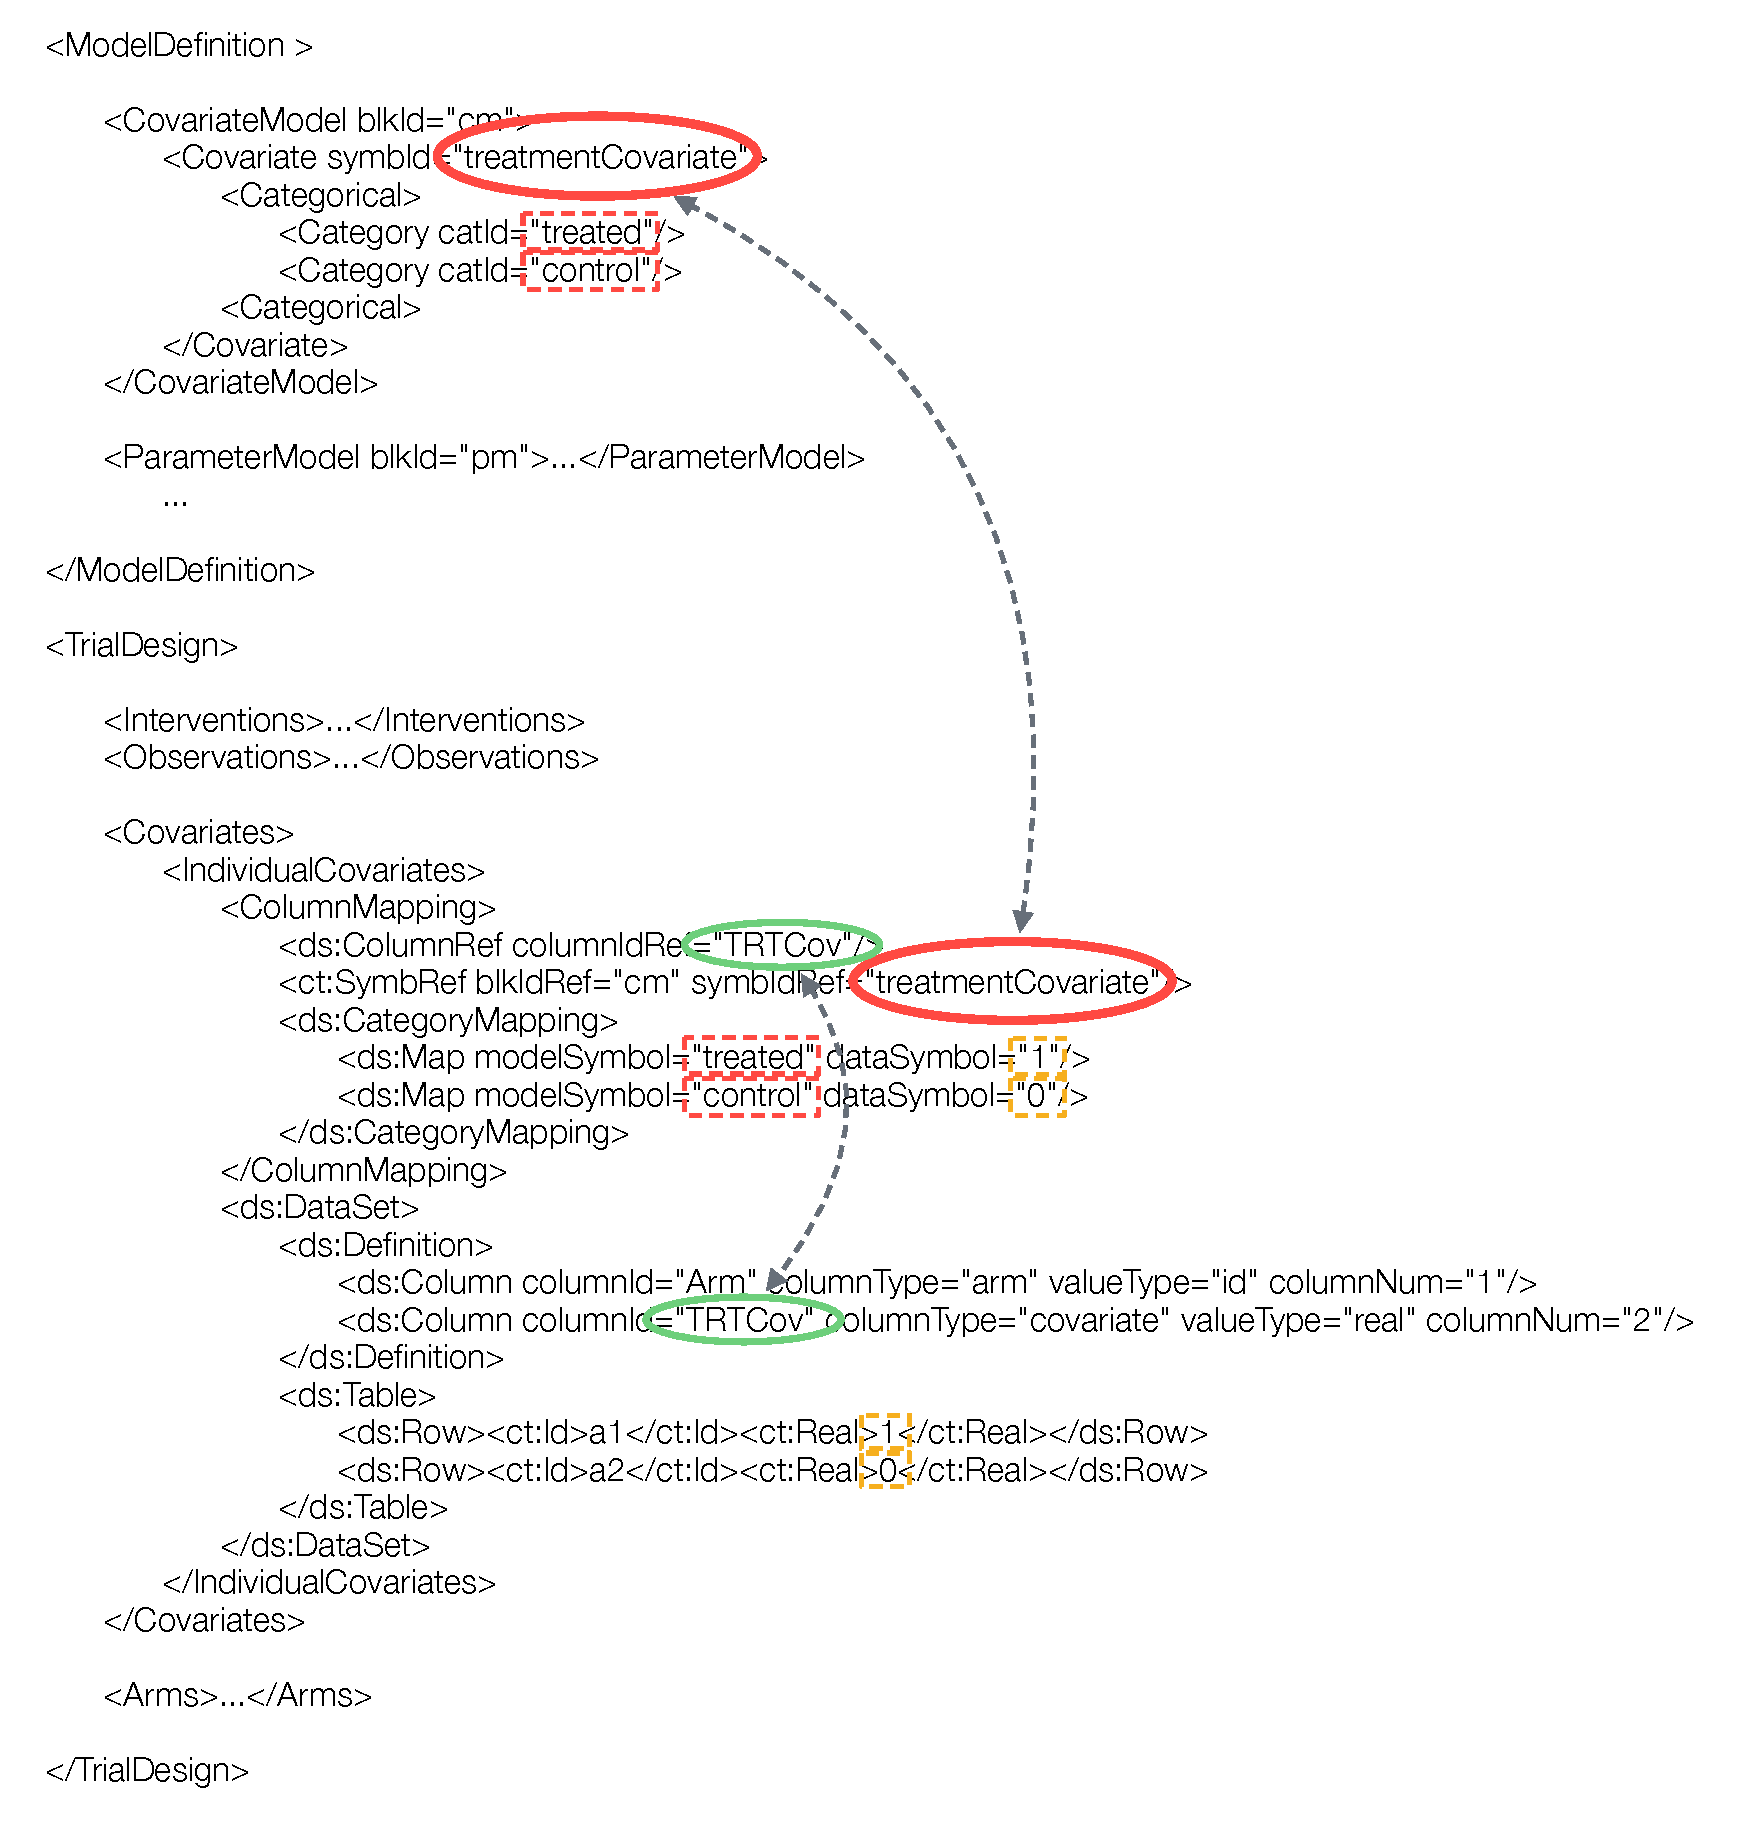
\includegraphics[width=130mm]{pics/Mapping_covariateModels_0_9}
  \caption{An example of how covariate are handled when they are encoded
  explicitly in the trial design using the \xelem{IndividualCovariates} element.}
  \label{fig:mapIndCov}
\end{figure}


%%%%%%%%%%%%%%%%%%%%%%%%%%%%
\subsubsection{Defining covariates}
\label{subsubsec:defCovariates}
In version $\le 0.8.1$ declaration of covariates was permitted only in the 
top level of the trial design, which posed a limitation on models. 
This restriction is now removed as the following section will show.
For more examples, see section \ref{sec:IOVinODE}.


%%%%%%%%%%%%%%%%%%%%%%%%%%%%
\subsubsection{Referencing covariates}
The above general example can be extended to cases when covariates are defined
per subject/arm, using the \xelem{IndividualCovariates} element, and when covariates
are associated with all arms or arm-wise.

The first snippet illustrates a case when both a covariate model, \xatt{td\_cm1}, and individual
covariates, \xatt{indivCov}, are defined.

\lstset{language=XML}
\begin{lstlisting}
    <TrialDesign>
        <Covariates>
            <CovariateModel oid="td_cm1">
                <!-- ... -->
            </CovariateModel>
            
            <IndividualCovariates oid="indivCov">
                <!-- omitted mapping -->
                <ds:DataSet>
                    <ds:Definition>
                        <ds:Column columnId="ID" columnType="id" valueType="string" columnNum="1"/>
                        <ds:Column columnId="ARM" columnType="arm" valueType="id" columnNum="2"/>
                        <ds:Column columnId="covariate1" columnType="covariate" valueType="string" columnNum="3"/>
                        <ds:Column columnId="covariate2" columnType="covariate" valueType="string" columnNum="4"/>
                        <!-- omitted other covariates -->
                    </ds:Definition>
                    <!-- omitted inline covariates records or external file reference -->
                </ds:DataSet>
            </IndividualCovariates>
        </Covariates>
\end{lstlisting}

These can then be referenced in the design arms in 
\begin{itemize}
\item 
the arms top level
\lstset{language=XML}
\begin{lstlisting}        
        <Arms>
            <CovariateModelRef oidRef="td_cm1"/>
            <!-- OR -->
            <IndividualCovariateRef oidRef="indivCov"/> 
            
            <Arm oid="arm1">
            	<!-- omitted interventions, observations etc. -->
		<!-- no covariate declarations here needed-->
            </Arm>
            <Arm oid="arm2">
            	<!-- omitted interventions, observations etc. -->
		<!-- no covariate declarations here needed-->
            </Arm>
\end{lstlisting}
\item 
or arm-wise -- here we assume further that individual covariates has been 
defined for each arm separately, as \xatt{indivCov1} and \xatt{indivCov2}, respectively
\lstset{language=XML}
\begin{lstlisting}
        <Arms>
            <Arm oid="arm1">
                <IndividualCovariatesRef oidRef="indivCov1"/>
                <!-- OR -->
                <CovariateModelRef oidRef="td_cm1"/>            <!-- REF to CovariateModel if no adjustment is required-->
                
                <CovariateModel oid="cm_arm1">
                    <CovariateModelRef oidRef="td_cm1"/> 
                    <!-- arm 1 specific adjustments to covariate model -->
                </CovariateModel>
            </Arm>
            <Arm oid="arm2">
                <IndividualCovariatesRef oidRef="indivCov2"/>
                
                <CovariateModel oid="cm_arm2">
                    <CovariateModelRef oidRef="td_cm1"/>
                    <!-- arm 2 specific adjustments to covariate model -->
                </CovariateModel>
                
            </Arm>
        </Arms>
    </TrialDesign>
\end{lstlisting}

\end{itemize}

%\subsubsection{Note on \xatt{columnType="covariate varLevel"}}
%While the double value assignment for the \xatt{columnType} attribute
%was designed to help in encoding and evaluating SO files, \cite{SO:2016b}, 
%it turns out to be useful here as well.
%
%Here, it identifies the EPOCH column as a covariate and variability level related.
%It must therefore be mapped to both the covariate model and the occasion 
%level of variability structure.


%add version with CModel
%\lstset{language=XML}
%\begin{lstlisting}
%        <CovariateModel blkId="td_cm1">
%            <CovariateModelRef blkIdRef="cm1"/>
%            <Covariate symbId="treatmentCovariate">
%                <mdef:Categorical>
%                    <ct:Assign>
%                        <math:Piecewise>
%                            <math:Piece>
%                                <ct:CatRef catIdRef="treated"/>
%                                <math:Condition>
%                                    <math:LogicBinop op="eq">
%                                        <StudyArm/> 
%                                        <math:ArmRef oidRef="a1"/>
%                                    </math:LogicBinop>
%                                </math:Condition>
%                            </math:Piece>
%                            <math:Piece>
%                                <ct:CatRef catIdRef="control"/>
%                                <math:Condition>
%                                    <math:LogicBinop op="eq">
%                                        <StudyArm/>
%                                        <math:ArmRef oidRef="a2"/>
%                                    </math:LogicBinop>
%                                </math:Condition>
%                            </math:Piece>
%                        </math:Piecewise>
%                    </ct:Assign>
%                </mdef:Categorical>
%            </Covariate>
%        </CovariateModel>	
%\end{lstlisting}



%%%%%%%%%%%%%%%%%%%%%%%%%%%%%
%\subsubsection{Referencing individual covariates}
%\label{subsec:refIndivCov}
%
%Declaration of the object identifier, attribute \xatt{oid}, is now
%mandatory as the example shows
%\lstset{language=XML}
%\begin{lstlisting}
%            <IndividualCovariates oid="ic1">
%                <ds:DataSet>
%                    <ds:Definition>
%                        <ds:Column columnId="ID" valueType="real" columnNum="1"/>
%                        <ds:Column columnId="WT" valueType="real" columnNum="2"/>
%                    </ds:Definition>
%                    <ds:ExternalFile oid="ef1">
%                        <ds:path>myIndivCovariates.csv</ds:path>
%                    </ds:ExternalFile>
%                </ds:DataSet>
%            </IndividualCovariates>
%\end{lstlisting}
%allowing referencing of individual covariates and covariate models
%in tasks, e.g. here in the estimation task
%
%\lstset{language=XML}
%\begin{lstlisting}
%        <EstimationStep oid="dsdas">
%	    ...
%            <!-- new reference element -->
%            <CovariatesReference>
%                <ct:OidRef oidRef="ic1"/>
%            </CovariatesReference>
%            ...
%\end{lstlisting}


%%%%%%%%%%%%%%%%%%%%%%%%%%%%%
%\subsubsection{Covariate model reference}
%
%\begin{itemize}
%\item 
%in model definition
%\lstset{language=XML}
%\begin{lstlisting}
%					<CovariateModelRef blkIdRef="cm1"/>
%\end{lstlisting}
%\item 
%in trial design
%\lstset{language=XML}
%\begin{lstlisting}
%					<CovariateModelRef oidRef="td_cm1"/>
%\end{lstlisting}
%\end{itemize}



%%%%%%%%%%%%%%%%%%%%%%%%%%%%%%%%%%%%%%%%%%%%%%%%%%%%%%%%%%%%%%%%%%%%%%
\section{Modelling steps}
\label{sec:modelSteps}

\subsection{Missing variable assignment added}
\xelem{VariableAssignment} has been added to the optimal design tasks
and can now be used to assign values to any model parameter or
variable similarly to what was possible in estimation or simulation tasks.


\subsection{Tool-specific settings}

\begin{itemize}
\item
The declaration of tool specific settings is now possible with new \xatt{tool} attribute in \xelem{Operation}
\end{itemize}

\lstset{language=XML}
\begin{lstlisting}
    <ModellingSteps xmlns="http://www.pharmml.org/pharmml/0.9/ModellingSteps">
        
            <!-- omitted elements -->
            
            <ParametersToEstimate>
                <ParameterEstimation>
                    <ct:SymbRef symbIdRef="d"/>
                    <InitialEstimate fixed="false">
                        <ct:Real>1</ct:Real>
                    </InitialEstimate>
                </ParameterEstimation>
                <!-- omitted elements -->
            </ParametersToEstimate>
            
            <Operation tool="Monolix" opType="estPop">
                <Algorithm definition="SAEM"/>
            </Operation>
            
            <Operation tool="NONMEM" opType="estPop">
                <Algorithm definition="FOCE"/>
            </Operation>
            
        </EstimationStep>
\end{lstlisting}


%%%%%%%%%%%%%%%%%%%%%%%%%%%%%%%%%%%%%%%%%%%%%%%%%%%%%%%%%%%%%%%%%%%%%%
\section{Other changes}
\label{sec:otherChanges}

\subsection{List of minor changes}

\begin{itemize}
\item 
new elements \xelem{Action}, \xelem{Combination}, \xelem{Intervention}
\xelem{Observation}, \xelem{Occasion}, \xelem{StudyArm} added -- allowing 
for conditioning of these trial design elements if required. See section \ref{subsec:condTrialDesingElems}
for an application example
\item
\xatt{CatRef} element added to operations
\item
imaginary unit $i$ added -- mathematical constant which is the square root of -1
\item
made order optional in \xelem{Operation}
\end{itemize}

\subsection{Dataset -- new column types}
\label{subsec:dataSets}
To provide the support for Monolix specific column types, 
following values have can be now assigned to the \xatt{columnType} 
attribute
\begin{itemize}
\item 
\emph{DATE} (or \emph{DAT1}, \emph{DAT2}, \emph{DAT3}) -- used to time stamp
\item 
\emph{YTYPE} -- response type identifier
\end{itemize}
see the Monolix specification for details.


%
%\subsection{Bugs fixes in Bayesian examples}
%
%PopulationParameter instead of RandomVariable in $lPOP\_P$ etc.
%IndividualParameter instead of PopulationParameter in  334 for 'lP'
%
%
